%----------------------------------------------------------------------------
\chapter*{\koszonetnyilvanitas}\addcontentsline{toc}{chapter}{\koszonetnyilvanitas}
%----------------------------------------------------------------------------
Szeretném őszinte hálámat és köszönetemet kifejezni belső konzulensemnek, Paál Dávidnak, aki a szakdolgozat
megírásában nyújtott felbecsülhetetlen segítségével, szakértelmével és támogatásával végigkísért.
Külső konzulensemnek, Tamás Dávidnak szintén mély hálával tartozom az általa munkámra szánt számos óráért, 
amelyeket gondos átnézésre, hasznos visszajelzések adására fordított, és hálás vagyok türelméért, valamint megértéséért. Valamint
megtiszteltetés volt számomra, hogy ez a hangrendszer a szakdolgozatom keretein belül valósulhatott meg.

Köszönetet szeretnék mondani a TéDé Rendezvényeknél dolgozó kollégáimnak is, akik minden ötletemet, 
legyen az bármilyen különleges, támogatták, és segítettek azok megvalósításában. A közös munka eredménye önmagáért beszél
a sok pozitív visszajelzés és sikeres rendezvény után.
%----------------------------------------------------------------------------
\begin {figure}[h!]
    \centering
    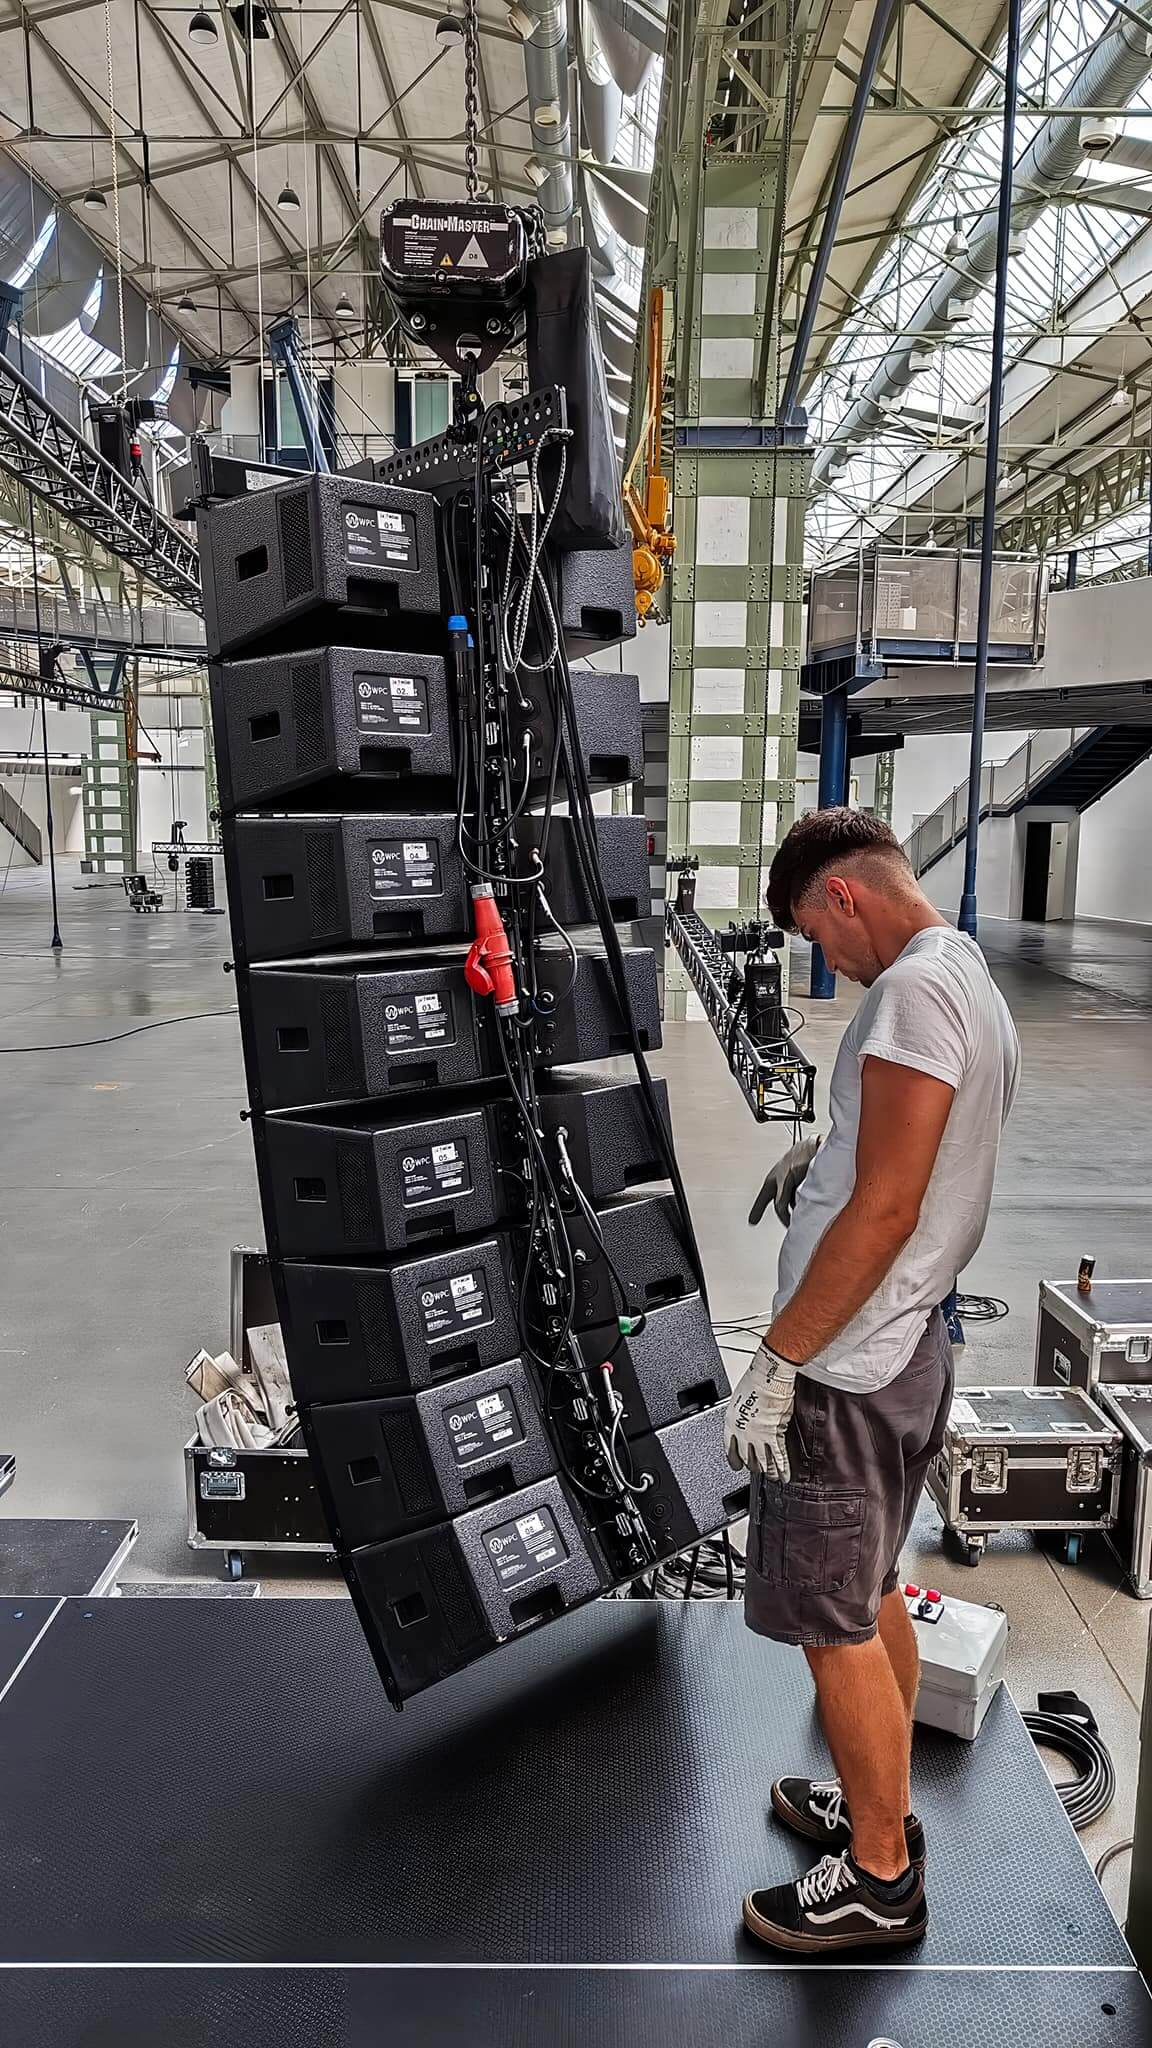
\includegraphics[width=0.5\textwidth]{figures/danci_wpc.jpg}
    \caption{A szakdolgozat szerzője a megépített WPC Line Array mögött az adott rendezvényen}
\end {figure}
%----------------------------------------------------------------------------
A csapattal végzett munkából szerzett tapasztalatok és élmények értékes betekintést nyújtottak a mérnöki 
szakma gyakorlati oldalába. Rávilágítottak arra, hogy a valóságban gyakran másképp alakulnak a dolgok, mint ahogy azt a tervezés során elképzeljük. 
Megtanultam alkalmazkodni, gyorsan reagálni a változásokra és kihívásokra, valamint nagy hangsúlyt fektetni a csapatmunkára. 
Emellett lehetőséget kaptam arra is, hogy szakdolgozatomhoz releváns adatokat gyűjtsek és felhasználjak, 
továbbá a sok raktári workshop nélkül a dolgozat nem jöhetett volna létre. 
Támogatásuk és bátorításuk a projekt minden szakaszában rendkívül értékes volt.

Végezetül, de nem kevésbé fontos módon, szeretném megköszönni minden barátomnak és 
családtagomnak a szakdolgozatom elkészítése során nyújtott állandó támogatásukat és bátorításukat. 
Értékes meglátásaik és építő jellegű visszajelzéseik kulcsszerepet játszottak a szakdolgozat sikerében. 
Hálás vagyok az irántam tanúsított kitartó támogatásukért és biztatásukért ezen az úton.